\documentclass{article}%
\usepackage[T1]{fontenc}%
\usepackage[utf8]{inputenc}%
\usepackage{lmodern}%
\usepackage{textcomp}%
\usepackage{lastpage}%
\usepackage[head=40pt,margin=0.5in,bottom=0.6in]{geometry}%
\usepackage{graphicx}%
%
\title{\textbf{Canasta Alimentaria de octubre se ubicó en Bs.S 52.322,32}}%
\author{Diario El Universal}%
\date{20/11/2018}%
%
\begin{document}%
\normalsize%
\maketitle%
\textbf{URL: }%
http://www.eluniversal.com/economia/26207/canasta{-}alimentaria{-}de{-}octubre{-}se{-}ubico{-}en{-}bss{-}5232232\newline%
%
\textbf{Periodico: }%
EU, %
ID: %
26207, %
Seccion: %
economia\newline%
%
\textbf{Palabras Claves: }%
NO\_TIENE\newline%
%
\textbf{Derecho: }%
2.10, %
Otros Derechos: %
, %
Sub Derechos: %
2.10.1\newline%
%
\textbf{EP: }%
NO\newline%
\newline%
%
\textbf{\textit{Según el Cendas, grasas y aceites aumentaron 278,7\% en octubre de 2018}}%
\newline%
\newline%
%
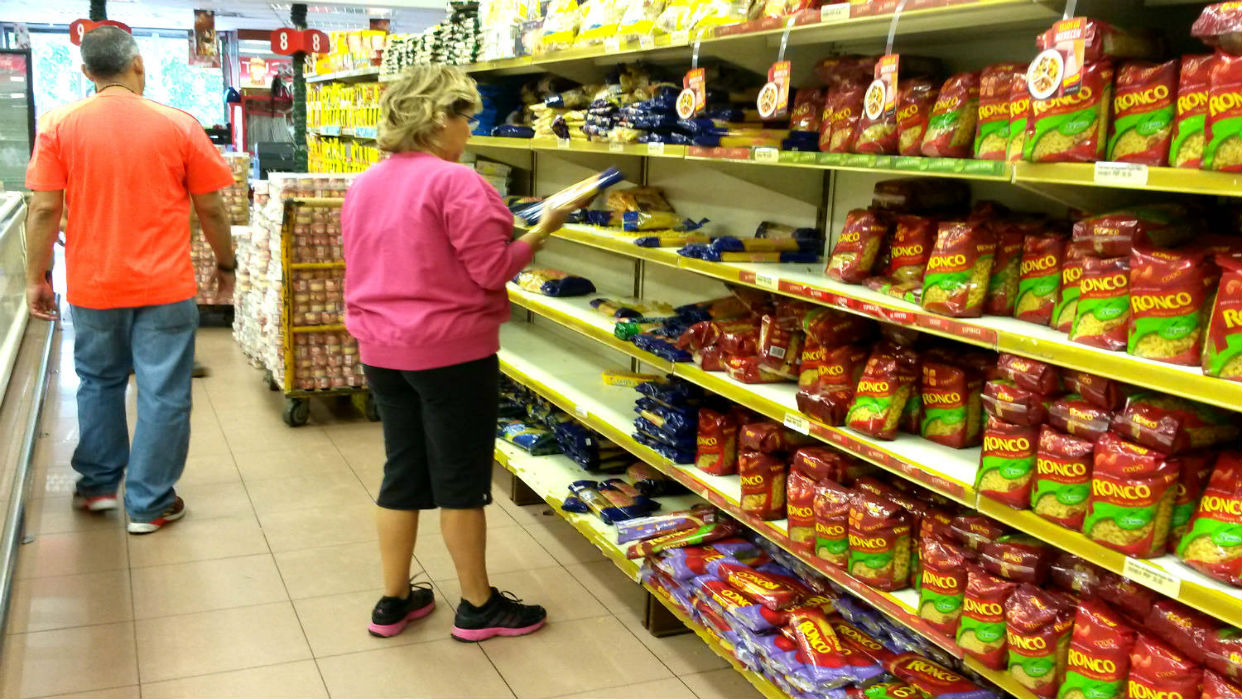
\includegraphics[width=300px]{29.jpg}%
\newline%
%
Caracas.{-}El precio de la Canasta Alimentaria Familiar del mes de octubre se ubicó en 52.322,32 bolívares soberanos, lo que representa un aumento de 128,3\% con respecto a septiembre que fue de 29.394,51 bolívares soberanos.%
\newline%
%
Betssy Santistevan Gastelú%
\newline%
%
Reportó en su informe mensual el Cendas{-}FVM.%
\newline%
%
Según la referida organización No gubernamental se requieren 29.1 salarios mínimos de Bs.S. 1.800,00, prácticamente un salario mínimo diario, para poder adquirir la referida canasta, a una familia de cinco miembros.%
\newline%
%
Señala el documento que todos los rubros de la canasta alimentaria aumentaron de precio: grasas y aceites, 278,7\%; carnes y sus preparados, 221,3\%; granos, 155,1\%; café, 127,6\%; frutas y hortalizas, 115,5\%; cereales y productos derivados, 111,4\%; leche, quesos y huevos, 103,6\%; pescados y mariscos, 79,9\%; raíces, tubérculos y otros, 76,3\%; azúcar y sal, 52,4\% y salsa y mayonesa, 45,9\%.%
\newline%
%
De este grupo, el rubro grasas y aceites subió de 408,03 a 1.545,25 bolívares soberanos, 278,7\%.%
\newline%
%
El aceite vegetal se vende en 395,13 bolívares soberanos el litro, 341,02 bolívares más, 630,2\%.  La margarina cuesta 179,93 bolívares soberanos, subió 57,08 bolívares soberanos, 46,5\%. \newline%
\newline%
El sector carnes y sus preparados subió 221,3\%, de Bs.S. 4.403,94 a 14.150,69.%
\newline%
%
La chuleta de cochino se vende en Bs.S. 2.957,50 el kilo, Bs.S. 2.389,03 más, 420,3\%.%
\newline%
%
El precio del pollo se incrementó en Bs.S. 360,60 el kilo, de Bs.S. 104,40 pasó a Bs.S. 465,00, 345,4\%. La carne para bisteck costaba Bs.S. 763,33 el kilo, Bs.S. 365,93 más, 92,1\%.  La carne de res molida y la de lagarto subieron Bs.S. 293,71, 77,0\%, de Bs.S. 381,29 a 675,00 el kilo.%
\newline%
%
El hígado de res subió Bs.S. 226,11, 72,8\%, de Bs.S. 310,55 a 536,66 el kilo.%
\newline%
%
El documento también destaca el precio de la Canasta Básica Familiar del décimo mes de 2018 es de 82.415,82 bolívares soberanos , lo que significa un aumento de 87,0\% frente el mes previo cuando se ubicó en Bs.S 22.927,8.%
\newline%
%
La variación de precios mensual de la Canasta Básica Familiar se debe al incremento de precio de todos los grupos que la integran.%
\newline%
%
En primer lugar, el alquiler de vivienda aumentó 670\%, de Bs.S 100,00 a 770,00\newline%
\newline%
El rubro de vestido y calzado aumentó Bs.S 2.078,61 al pasar de 5.410,25 a Bs.S 7.488,86; como promedio mensual, 38,4\%, se lee.%
\newline%
%
\end{document}